%%%%%% Run at command line, run
%%%%%% xelatex grad-sample.tex 
%%%%%% for a few times to generate the output pdf file
\documentclass[12pt,oneside,openright,a4paper]{cpe-english-project}

 \usepackage{polyglossia}
 \setdefaultlanguage{english}
 \setotherlanguage{thai}
\newfontfamily\thaifont[Script=Thai,Scale=1.23]{TH Sarabun New}
\defaultfontfeatures{Mapping=tex-text,Scale=1.0,LetterSpace=0.0}
\setmainfont[Scale=1.0,LetterSpace=0,WordSpace=1.0,FakeStretch=1.0]{Times New Roman}
\emergencystretch=10pt
%\XeTeXlinebreaklocale "th_TH"	
%\XeTeXlinebreakskip = 0pt plus 1pt
%\setmathfont(Digits)[Scale=1.0,LetterSpace=0,FakeStretch=1.0]{Times New Roman}


%%%%%%%%%%%%%%%%%%%%%%%%%%%%%%%%%%%%%%%%%%%%%%%%%%%%%%%%%%%%%%%%%%%
% Customize below to suit your needs 
% The ones that are optional can be left blank. 
%%%%%%%%%%%%%%%%%%%%%%%%%%%%%%%%%%%%%%%%%%%%%%%%%%%%%%%%%%%%%%%%%%%
% First line of title
\def\disstitleone{Writing Aid to Avoid Repetitions}   
% Second line of title
%\def\disstitletwo{Project/Indep title line 2 (optional)}   
% Your first name and lastname
\def\dissauthor{Mr.Annop Pornsawatdipak}   % 1st member
%%% Put other group member names here ..
\def\dissauthortwo{Mr.Thanapatr Amnuaywit}   % 2nd member (optional)
\def\dissauthorthree{Mr./Ms. Firstname3 Lastname3}   % 3rd member (optional)


% The degree that you're persuing..
\def\dissdegree{Bachelor of Engineering} % Name of the degree
\def\dissdegreeabrev{B.Eng} % Abbreviation of the degree
\def\dissyear{2022}                   % Year of submission
\def\thaidissyear{2565}               % Year of submission (B.E.)

%%%%%%%%%%%%%%%%%%%%%%%%%%%%%%%%%%%%%%%%%%%%
% Your project and independent study committee..
%%%%%%%%%%%%%%%%%%%%%%%%%%%%%%%%%%%%%%%%%%%%
\def\dissadvisor{Assoc.Prof. Nuttanart Muansuwan Facundes, Ph.D.}  % Advisor
%%% Leave it empty if you have no Co-advisor
\def\disscoadvisor{Assoc.Prof. My Co-advisor name, Ph.D.}  % Co-advisor
\def\disscommitteetwo{Asst.Prof. Committee2, Ph.D.}  % 3rd committee member (optional)
\def\disscommitteethree{Asst.Prof. Committee3, Ph.D.}   % 4th committee member (optional) 
\def\disscommitteefour{}    % 5th committee member (optional) 

\def\worktype{Project} %%  Project or Independent study
\def\disscredit{3}   %% 3 credits or 6 credits


\def\fieldofstudy{Computer Engineering} 
\def\department{Computer Engineering} 
\def\faculty{Engineering}

\def\thaifieldofstudy{วิศวกรรมคอมพิวเตอร์} 
\def\thaidepartment{วิศวกรรมคอมพิวเตอร์} 
\def\thaifaculty{วิศวกรรมศาสตร์}
 
\def\appendixnames{Appendix} %%% Appendices or Appendix

\def\thaiworktype{ปริญญานิพนธ์} %  Project or research project % 
\def\thaidisstitleone{โปรแกรมช่วยเขียนโดยหลีกเลี่ยงคำซ้ำ}
%\def\thaidisstitletwo{หัวข้อปริญญานิพนธ์บรรทัดสอง}
\def\thaidissauthor{นายอรรณพ พรสัวสดิภักดิ์}
\def\thaidissauthortwo{นายธนภัทร อำนวยวิทย์} %Optional
\def\thaidissauthorthree{นางสาวสมปอง คอมพิวเตอร์3} %Optional

\def\thaidissadvisor{ผศ.ดร.ณัฐนาถ เหมือนสุวรรณ}
%% Leave this empty if you have no co-advisor
\def\thaidisscoadvisor{รศ.ดร.ที่ปรึกษา วิทยานิพนธ์ร่วม} %Optional
\def\thaidissdegree{วิศวกรรมศาสตรบัณฑิต}

% Change the line spacing here...
\linespread{1.15}

%%%%%%%%%%%%%%%%%%%%%%%%%%%%%%%%%%%%%%%%%%%%%%%%%%%%%%%%%%%%%%%%
% End of personal customization.  Do not modify from this part 
% to \begin{document} unless you know what you are doing...
%%%%%%%%%%%%%%%%%%%%%%%%%%%%%%%%%%%%%%%%%%%%%%%%%%%%%%%%%%%%%%%%


%%%%%%%%%%%% Dissertation style %%%%%%%%%%%
%\linespread{1.6} % Double-spaced  
%%\oddsidemargin    0.5in
%%\evensidemargin   0.5in
%%%%%%%%%%%%%%%%%%%%%%%%%%%%%%%%%%%%%%%%%%%
%\renewcommand{\subfigtopskip}{10pt}
%\renewcommand{\subfigbottomskip}{-5pt} 
%\renewcommand{\subfigcapskip}{-6pt} %vertical space between caption
%                                    %and figure.
%\renewcommand{\subfigcapmargin}{0pt}

\renewcommand{\topfraction}{0.85}
\renewcommand{\textfraction}{0.1}

\newtheorem{theorem}{Theorem}
\newtheorem{lemma}{Lemma}
\newtheorem{corollary}{Corollary}

\def\QED{\mbox{\rule[0pt]{1.5ex}{1.5ex}}}
\def\proof{\noindent\hspace{2em}{\itshape Proof: }}
\def\endproof{\hspace*{\fill}~\QED\par\endtrivlist\unskip}
%\newenvironment{proof}{{\sc Proof:}}{~\hfill \blacksquare}
%% The hyperref package redefines the \appendix. This one 
%% is from the dissertation.cls
%\def\appendix#1{\iffirstappendix \appendixcover \firstappendixfalse \fi \chapter{#1}}
%\renewcommand{\arraystretch}{0.8}
%%%%%%%%%%%%%%%%%%%%%%%%%%%%%%%%%%%%%%%%%%%%%%%%%%%%%%%%%%%%%%%%
%%%%%%%%%%%%%%%%%%%%%%%%%%%%%%%%%%%%%%%%%%%%%%%%%%%%%%%%%%%%%%%%


\begin{document}
\pdfstringdefDisableCommands{%
\let\MakeUppercase\relax
}
\begin{center}
  
\includegraphics[width=2.8cm]{logo02.jpg}
\end{center}
\vspace*{-1cm}

\maketitlepage
\makesignaturepage 

%%%%%%%%%%%%%%%%%%%%%%%%%%%%%%%%%%%%%%%%%%%%%%%%%%%%%%%%%%%%%%
%%%%%%%%%%%%%%%%%%%%%% English abstract %%%%%%%%%%%%%%%%%%%%%%%
%%%%%%%%%%%%%%%%%%%%%%%%%%%%%%%%%%%%%%%%%%%%%%%%%%%%%%%%%%%%%%
\abstract

The computer-assisted writing aims to help improve the quality of a piece of text with the help of computer. Most of the tools focus on fixing grammatical accuracy and misspelled words, only few of them offer repetition detectors. In this project we will be creating a program to keep track of the words and phrases frequency. Moreover, our program will suggest alternative words that fits in original context, thus, the writer can replace the word marked as repetitive with a new suggested word instead. Our proposed solutions consisted of two main parts, the detector, and the suggestor. In the first part, the program tries to detect only relevant repetitions and filter out very specific words or very trivial words. Next, the suggestor module will generate multiple substitution candidates by feeding the sentence into the Transformer model. The transformer model such as BERT is trained with Masked Language Modelling, which we can use to predict the mask position, in this case the target word to replace. The generated candidates are verified using SentenceBERT and similarity score to ensure each of them won’t alter the meaning of the original sentence. 

\begin{flushleft}
\begin{tabular*}{\textwidth}{@{}lp{0.8\textwidth}}
\textbf{Keywords}: & Overused word detector / repetitive word detector / BERT / NLP
\end{tabular*}
\end{flushleft}
\endabstract

%%%%%%%%%%%%%%%%%%%%%%%%%%%%%%%%%%%%%%%%%%%%%%%%%%%%%%%%%%%%%%
%%%%%%%%%% Thai abstract here %%%%%%%%%%%%%%%%%%%%%%%%%%%%%%%%%
%%%%%%%%%%%%%%%%%%%%%%%%%%%%%%%%%%%%%%%%%%%%%%%%%%%%%%%%%%%%%%
{
%\begin{thai}
\XeTeXlinebreaklocale "th_TH"	
\XeTeXlinebreakskip = 0pt plus 1pt
\thaifont
\thaiabstract

การเขียนโดยใช้คอมพิวเตอร์เป็นตัวช่วยมีจุดมุ่งหมายเพื่อช่วยปรับปรุงคุณภาพของข้อความโดยใช้คอมพิวเตอร์เข้ามาช่วยเหลือ เครื่องมือส่วนใหญ่มุ่งเน้นไปที่การแก้ไขความถูกต้องทางไวยากรณ์และคำที่สะกดผิด มีเพียงไม่กี่เครื่องมือเท่านั้นที่มีระบบตรวจจับคำซ้ำ ในโครงการนี้ เราจะสร้างเครื่องมือเพื่อติดตามความถี่ของคำและวลี นอกจากนี้ โปรแกรมของเราจะแนะนำคำทดแทนที่เหมาะกับบริบทเดิม ดังนั้น ผู้เขียนสามารถแทนที่คำที่ถูกทำเครื่องหมายว่าซ้ำด้วยคำใหม่ที่แนะนำแทน แนวทางที่เรานำเสนอประกอบด้วยสองส่วนหลัก ได้แก่ ตัวตรวจจับ และตัวแนะนำ ในส่วนแรก โปรแกรมจะพยายามตรวจหาเฉพาะคำซ้ำที่เกี่ยวข้องและกรองคำเฉพาะหรือคำที่ไม่สำคัญออก ถัดไป โมดูลผู้แนะนำจะสร้างชุดคำทางเลือกสำหรับทดแทน โดยป้อนประโยคลงในโมเดล Transformer โมเดลทรานสฟอร์เมอร์ เช่น BERT ได้รับการฝึกฝนด้วย Masked Language Modeling ซึ่งเราสามารถใช้มันเพื่อทำนายตำแหน่งของมาสก์ ในกรณีนี้ คำเป้าหมายที่จะแทนที่ คำทดแทนที่สร้างขึ้นจะได้รับการตรวจสอบโดยใช้ SentenceBERT และคะแนนความคล้ายคลึงกันเพื่อให้แน่ใจว่าแต่ละคำจะไม่เปลี่ยนความหมายของประโยคเดิม

\begin{flushleft}
\begin{tabular*}{\textwidth}{@{}lp{0.8\textwidth}}
 & \\

\textbf{คำสำคัญ}: & การตรวจจับคำที่ใช้บ่อย / การตรวจจับคำซ้ำ / BERT / NLP
\end{tabular*}
\end{flushleft}
\endabstract
%\end{thai}
}

%%%%%%%%%%%%%%%%%%%%%%%%%%%%%%%%%%%%%%%%%%%%%%%%%%%%%%%%%%%%
%%%%%%%%%%%%%%%%%%%%%%% Acknowledgments %%%%%%%%%%%%%%%%%%%%
%%%%%%%%%%%%%%%%%%%%%%%%%%%%%%%%%%%%%%%%%%%%%%%%%%%%%%%%%%%%
\preface
Acknowledge your advisors and thanks your friends here..

%%%%%%%%%%%%%%%%%%%%%%%%%%%%%%%%%%%%%%%%%%%%%%%%%%%%%%%%%%%%%
%%%%%%%%%%%%%%%% ToC, List of figures/tables %%%%%%%%%%%%%%%%
%%%%%%%%%%%%%%%%%%%%%%%%%%%%%%%%%%%%%%%%%%%%%%%%%%%%%%%%%%%%%
% The three commands below automatically generate the table 
% of content, list of tables and list of figures
\tableofcontents                    
\listoftables
\listoffigures                      

%%%%%%%%%%%%%%%%%%%%%%%%%%%%%%%%%%%%%%%%%%%%%%%%%%%%%%%%%%%%%%
%%%%%%%%%%%%%%%%%%%%% List of symbols page %%%%%%%%%%%%%%%%%%%
%%%%%%%%%%%%%%%%%%%%%%%%%%%%%%%%%%%%%%%%%%%%%%%%%%%%%%%%%%%%%%
% You have to add this manually..
\listofsymbols
\begin{flushleft}
\begin{tabular}{@{}p{0.07\textwidth}p{0.7\textwidth}p{0.1\textwidth}}
\textbf{SYMBOL}  & & \textbf{UNIT} \\[0.2cm]
$\alpha$ & Test variable\hfill & m$^2$ \\
$\lambda$ & Interarival rate\hfill &  jobs/second\\
$\mu$ & Service rate\hfill & jobs/second\\
\end{tabular}
\end{flushleft}
%%%%%%%%%%%%%%%%%%%%%%%%%%%%%%%%%%%%%%%%%%%%%%%%%%%%%%%%%%%%%%
%%%%%%%%%%%%%%%%%%%%% List of vocabs & terms %%%%%%%%%%%%%%%%%
%%%%%%%%%%%%%%%%%%%%%%%%%%%%%%%%%%%%%%%%%%%%%%%%%%%%%%%%%%%%%%
% You also have to add this manually..
\listofvocab
\begin{flushleft}
\begin{tabular}{@{}p{1in}@{=\extracolsep{0.5in}}l}
ABC & Adaptive Bandwidth Control \\
MANET & Mobile Ad Hoc Network 
\end{tabular}
\end{flushleft}

%\setlength{\parskip}{1.2mm}

%%%%%%%%%%%%%%%%%%%%%%%%%%%%%%%%%%%%%%%%%%%%%%%%%%%%%%%%%%%%%%%
%%%%%%%%%%%%%%%%%%%%%%%% Main body %%%%%%%%%%%%%%%%%%%%%%%%%%%%
%%%%%%%%%%%%%%%%%%%%%%%%%%%%%%%%%%%%%%%%%%%%%%%%%%%%%%%%%%%%%%%


\chapter{Introduction}

\section{Problem statement and Approach} 

Writing a long text such as an essay, or an academic report can be challenging, especially for non-native English speakers. One of the most common problems is the overuse of certain vocabulary, which can distract the readers and make the article less professional. With limited lexical resources, the writing may sound boring and can potentially weaken the message the writer wants to convey. Particularly in academic writing where the readers are highly educated, repetition is an undesirable trait and can be seen as disrespectful to the readers (Fosu, 2020\cite{fosu20}). This project will focus on helping non-native users of English to reduce repetitions in their writing which will improve the overall quality of their work.

\section{Objectives}
Keep track of overused words and suggest alternatives based on context.

\section{Project Scope}
\begin{itemize}
\item A working Windows application with Graphical User Interface (GUI)
\item An application consists of a text input area and a sidebar for suggestions and other related information.
\item Give suggestions for repetitive words/phrases only
\item Suggestion does not include grammatical corrections, such as verb tense, spelling, etc.
\item Supports English language only
\end{itemize}

\section{Project Schedule}
Term 1\\ \\
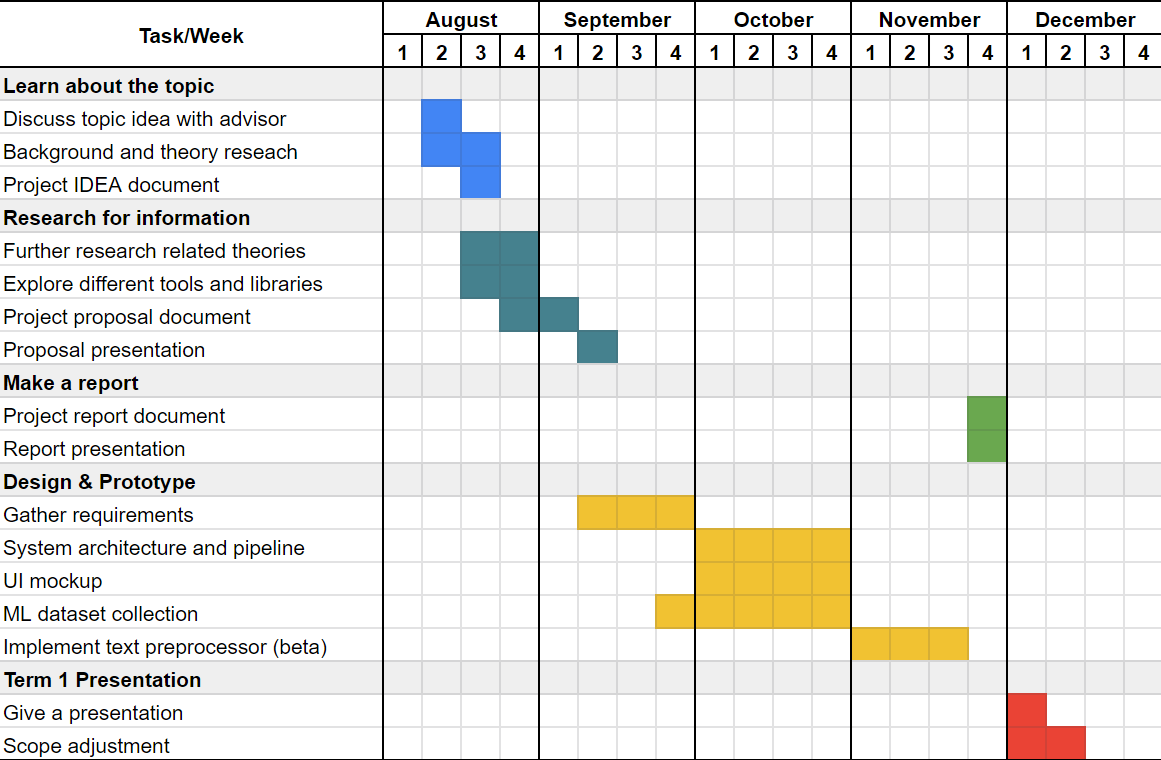
\includegraphics[width=15cm]{./img/chp1/schedule1.png}

Term 2\\ \\
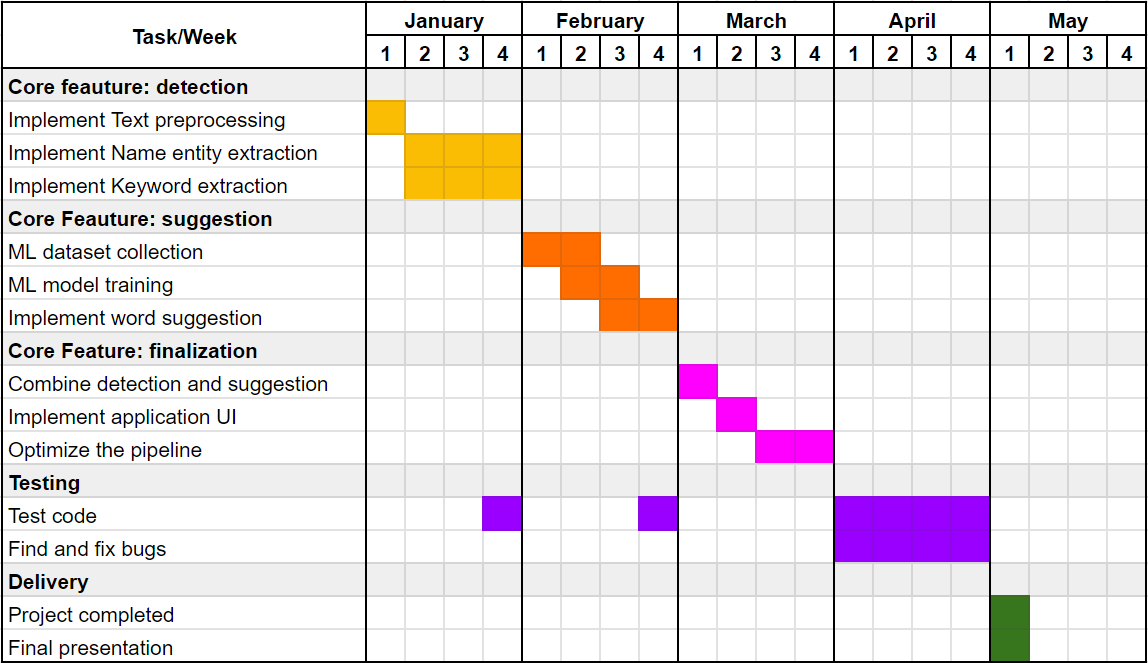
\includegraphics[width=15cm]{./img/chp1/schedule2.png}

Term 1\\
1. Learn about the topic
\begin{itemize}
\item Discuss topic idea
\item Define problem definition, scope and method
\item Make the IDEA document
\end{itemize}
2. Research for more information
\begin{itemize}
\item Further research related theories
\item Explore different tools and libraries
\item Make a final proposal and presentation   
\end{itemize} 
3. Design \& prototyping
\begin{itemize}
\item Gather requirements
\item Design system architecture and pipeline
\item Create an UI mockup
\item Try implementing text preprocessor
\end{itemize}
4. Term 1 final report and presentation\\


Term 2\\
1. Core feature: detection
\begin{itemize}
\item Implement Text Preprocessing
\item Implement Name Entity Extraction
\item Implement Keyword extraction
\end{itemize}
2. Core feature: suggestion
\begin{itemize}
\item Finish up ML datasets collecting process
\item ML model training
\item Implement word suggestion
\end{itemize}
3. Finalize the application
\begin{itemize}
\item Combine detection and suggestion
\item Optimize the pipeline
\item Implement application UI
\end{itemize}
4. Testing
\begin{itemize}
\item Application testing
\item Discover problems and errors
\item Fixing bugs
\end{itemize}
5. Delivery
\begin{itemize}
\item Complete the project
\item Final report and presentation
\end{itemize}


\section{Deliverables}
Term 1
\begin{enumerate}
\item Proposal
\item Project report(unfinished) and presentation
\item Requirement list
\item Text preprocessor (beta)
\item UI mockup
\item System architecture\\
\end{enumerate}

Term 2
\begin{enumerate}
\item Completed application
\item Completed project report
\end{enumerate}


%%%%%%%%%%%%%%%%%%%%%%%%%%%%%%%%%%%%%%%%%%%%%%%%%%%%%%%%%%%%
%%%%%%%%%%%%%%  Literature Review %%%%%%%%%%%%%%%%%%%%%%%%%%
%%%%%%%%%%%%%%%%%%%%%%%%%%%%%%%%%%%%%%%%%%%%%%%%%%%%%%%%%%%%
\chapter{Background Theory and Related Work}
\section{Background}
Writing an academic article in English poses a number of challenges to the writer, particularly those whose English is not their first language for example ESL students (English as Second Language) and EFL students (English as Foreign Language). There are a number of difficulties that often come up when writing a long piece of tex;t namely sentence structural problems, grammatical mistakes, coherence and cohesion. Nonetheless, one of the most prominent struggle writers face is having limited lexical resources which leads to the repetitive use of a certain word. The research regarding connector usage of Japanese EFL learners found that learners significantly overuse some connecting devices, especially sentence-initial positions. It also revealed that both native users and Japanese EFL students share a common set of high-frequency linking devices (Narita et al., n.d.). The researchers suggested some of the reasons for this problem include the lack of familiarity with the word and inadequate knowledge. Another investigation (Hama, 2021) supports the claim by pointing out a familiarity issue with certain connecting words which ultimately resulted in repetitive use of linking words. 

Repetition in an academic context is especially critical due to the audience being highly knowledgeable. As Fosu (2021) said, “Not only is repeating things distracting, but it’s also somewhat insulting to a person’s intelligence”. In certain scenarios, the issue arises due to the mindlessness of the writer rather than a lack of skill. As the text becomes longer, it is harder to keep track of how often a certain vocabulary has been used in the text, thus the repetition becomes more difficult to control. The writer can certainly read through the entire document to identify overuse words, however, this is a daunting task and time-consuming to re-read multiple times.

Natural Language Processing (NLP) has been greatly advanced in recent years both in terms of efficiency and accuracy. A state-of-art machine learning-based NLP has emerged thanks to tremendous textual data human generates each day. Currently, there are numerous services focused on computer-assited writing, for instance, Grammarly, Prowritingaid, Gramara, Microsoft Word’s Editor, Writer.com, and more. Most of them focus on fixing grammatical errors, typos, and punctuation, only a few of them offer overuse word detection. As mentioned above, we decided to create an application to help writers avoid repetition by keeping track of their word frequency as well as suggesting alternative words to use. The target user of this project is non-native English student writers in an academic context.
\section{Related Theory}
\subsection{Natural Language Processing}
Natural language Processing (NLP) is a sub-field of computer science (also a branch of Artificial intelligence depending on the technique used) defined as a way to give computers the ability to understand text and spoken language in the same way human beings can (IBM, 2020). According to IBM,  NLP is a multidisciplinary combining computational linguistics, rule-based modeling of human language, statistics, machine learning, and deep learning models. All of these enable computers to interpret natural language in both textual and verbal forms.  NLP has various use cases both for personal and business use such as machine translators, voice-activated speakers, virtual assistants, virtual agents, customer service chatbots, and social media analysis respectively. Early, NLP applications often rely on a rule-based approach which means the programmer must hard code all the linguistic rules to let the computer perform NLP tasks. However, human language is full of ambiguity and exceptions which makes traditional methods cannot scale to capture all the nuance of everchanging human language. Thus, most modern-day NLP applications let the computer learn patterns by themself using Machine Learning instead.
\subsubsection{Part-of-speech Tagging}
A process of assigning the part of speech to different words in a piece of text. Part of speech is critical as some words can be both verb and noun depending on the usage for example “ship” in the product has been shipped or “ship” in the ship will not float.

\subsubsection{Word sense disambiguation}
A method to determine which meaning to use in a certain context in case the word has more than one meaning. For example, “park” could mean a large public green area or bring a vehicle to a halt and leave it temporarily. This can be done through semantic analysis.

\subsubsection{Name entity recognition}
A technique used to automatically identify name and location in the given text, for instance, Steve Jobs was kicked out of Apple, here, Steve Jobs is a person, and Apple is a company.

\subsubsection{Sentiment analysis}
An attempt to interpret the tone and attitude of the text. Useful for detecting emotions, sarcasm, confusion, and suspicion in the text.

\subsubsection{Natural Language Generation}
A process where computers create textual information that humans can understand.

\subsubsection{Keyword Extraction}
A method used to automatically find the most relevant words and phrases from a piece of document. Allowing the computer to know the main idea of the text. Some of the most well-known techniques (Pradeep, 2022) are KeyBERT, Rapid Automatic Keyword Extraction (aka. Rake), Yet Another Keyword Extractor (aka. YAKE), and TextRank.

\subsection{Pointwise Mutual Information}
Pointwise Mutual Information (PMI) is a technique used to analyze the association between words. PMI asks how much more the two words co-occur in our corpus than we would have a prior expected them to appear by chance (Jurafsky, 2021). PMI permits the ability to detect word pairs that occur together, thus, is useful when performing a cooccurrence analysis of words in the corpus. The formula is as follows.

\subsection{Likelihood ratio}
	According to packtpub.com(n.d.), likelihood ratio or log-likelihood ratio is a measure of how two events are unlikely to be independent but occur together more than by chance. This is used to measure the level of association between tokens, aka. bigram, trigram. A higher score indicates a significant co-occurrence between those tokens. Unlike PMI, this metric is not biased toward low-frequency words.

\subsection{Byte-pair encoding (BPE)}
A type of tokenizer where the word is broken down into tokens each containing a single character. A token can be merged to form a larger group. Similarly, each group can also be joined together to form a word. 
Example: This is tokenizing -> T h i s i s t o k e n i z i n g -> this is token izing

\subsection{Attention}
Traditional sequence to sequence approaches such as LSTM and RNN tend to suffer from the vanishing gradient problem, where the model failed to capture long term dependencies in a lengthy text. The attention model comes to solve this problem as it permits the model to focus on only the important information of the input. Instead of encoding the entire input sentence into a fixed-sized vector, the model learned to attend to parts of the sentence that are relevant to the output it will produce.  The decoder performs additional before outputting the result which is 1) look at each hidden state received from the encoder, 2) assign each of them a score, 3) apply softmax to each score, thus, higher scores will be amplified, the lower scores will be suppressed.

\subsection{Transformer}
According to the paper called “Attention is all you need”, published in 2017, the author purposed an encoder-decoder architecture based on attention layers which was later known as the transformer. Initially, the transformer is intended to be used in the translation field, but due to its performance, scalability and versatility, this method is widely adopted by the research community and enterprise to solve challenging NLP tasks. Unlike LSTM or RNN, where it can only process words in a sentence sequentially as dictated by the design. The encoder-decoder architecture processes input in parallel manners. 

\subsubsection{Input Embedding [1]}
Textual input must be converted into a vector or in NLP, we called it an embedding. Every word is represented as a vector of values corresponding to its meanings. 

\subsubsection{Positional Encoding [2]}
Due to its parallelism property, each word in a sentence will get through the model simultaneously which means it doesn't know what order they are in. The positional encoding assigns each embedding a vector denoting its position.

\subsubsection{Multi-headed attention [3]}
This mechanism allows the model to pay attention to a specific token in the input. The attention vector captures the relationship between each word to the other words in the sentence. In self-attention, the model will give more weight to itself. However, this is not ideal because we are interested in obtaining the interaction between words. So instead, there are multiple attention heads per word which will be averaged out to get the final attention vector for every word.

\subsubsection{Add and Norm [4]}
Normalization is performed on each output layer-wise.

\subsubsection{Feed Forward [5]}
A feed-forward neural network is applied to every attention vector. This will transform the attention vector into a suitable format for the decoder/encoder block. All the vectors are passed to the network parallelly.

\subsubsection{Masked multi-headed attention [6]}
The multi-headed attention block generates attention vectors for every word in the sentence and the take average to get the final attention vector denotes the relationship between words. This resembles multi-headed attention but now included masks.
The reason is to prevent the model from having access to the future token that has not appeared yet in the natural ordering of the sentence. Mask is essentially to replace those positions with zero. Thus, the attention score will be computed in accordance with the previous token only and not the future one. 

\subsubsection{Multi-head attention [7]}
The attention vectors and the vector from the encoder are passed to the block similar to the previous one except now the input is coming from the encoder. So, we may refer to it as an encoder-decoder attention block. This block contains vectors for both languages and this is where the mapping between the 2 languages takes place. The output is in a form of attention vectors representing the relationship of words from both languages. 

\subsubsection{Linear [8]}
A kind of feed-forward network expands the multi-headed attention output to the dimension of size equal to the vocabulary in the target language. 

\subsubsection{Softmax [9]}
Calculate the probability score ranging from 0 to 1 for every class (words in the language). The class with the highest probability will be selected as the final output.

\section{Technologies and Development Tools}
\subsection{Python} 
Python is an object-oriented programming language that supports a wide selection of libraries including PyTorch, Spacy, NLTK, etc. 
 
\subsection{PyTourch} 
A machine learning library written in python.

\subsection{Natural Language Toolkit (NLTK)} 
A toolkit provides some of the basic operations in NLP including stemming, tokenization, cooccurrence analysis, etc. 

\subsection{Spacy} 
A more advanced NLP library shipped with several ready-to-use tools such as tokenizer, NER, POS, Lemmatizer, and Training pipeline.  

\subsection{Tkinter} 
A GUI builder for Python applications. Provide basic tools to create GUI elements such as a window, a button, an input field, etc. 

\subsection{Visual Studio Code} 
A code editing software from Microsoft. Supports a wide range of plugins and add-ons which help streamline the development process. Collaborative code editing allows teammates to work on the same project remotely anytime anywhere. 

\subsection{Matplotlib} 
A library to help visualize results as a graphical representation such as confusion matrix, correlation plot, performance analysis, etc. 



\subsection{Huggingface Transformer} 
An open-source library dedicated to the development of NLP applications using transformers. It is compatible with both Tensorflow and PyTorch. The package includes numerous state-of-the-art models including BERT, Roberta, XLNet, T5, and more. It also supports various NLP pipelines for performing different tasks out-of-the-box some of them are audio classification, question answering, summarization, and translation. Moreover, this library provides a range of utility functions for training, finetuning, inferencing, etc.


\section{Related Research}
\subsection{Embedding Dropout}
As mentioned, BERT has been trained using masked language modeling, it is capable of predicting a masked token of the sentence. However, if we feed the sentence where a word is replaced with <masked> token, the predicted token will likely fit in the context but may not retain its original meaning. According to Zhou, et al., the embedding dropout can be used to overcome this issue. It is the technique where the random index of the token will be set to zero, thus, it allows the model to get partial information about the target word but help avoid overfitting. This approach helps improve the performance of the prediction according to the researcher. Further evaluation of performance when implemented in our project is needed.

\subsection{Sentence Concatenation}
According to the article, A simple BERT-Based Approach for Lexical Simplication purposed by Jipeng et al. The research focuses on simplifying complex words, although not directly related, this method is applicable to our project. The authors state that considering the complex word w in sentence S, the word w is masked to create a new sentence S’ and feed into the model. By doing this, the model will not consider the influence of the complex word.  To give some clue about the target word, the sentence with a masked token will be concatenated with the original sentence that has no mask. Both sentences are then passed into the model to get the prediction. This allows the model to get some contexts about the target words, therefore, the output will be relatively close to the target word. 

\subsection{BERT}
Based on Bidirectional Encoder Representations from Transformer (aka. BERT), A machine learning-based approach purposed by Google AI Language (Horev, 2018). It achieved superior performance by reading the entire sequence of words at once, instead of left to right or right to left like most of the previous works. This allows the model to learn the context of words using clues from their surroundings. BERT has been trained using 2 objectives in mind. The first is called next-sentence prediction where it tries to predict whether the given sentence will follow the previous sentence or not. Next, the masked language model where the random part of the corpus is masked and the model tries to fill in the gap. This research has become one of the best-performing approaches in the NLP world. Despite that, the model itself is inefficient and slow to run due to the complexity, so in this project, we decided to use another model named Roberta. At its core, Roberta is similar to BERT but without the Next sentence prediction objective, which noticeably improves the execution speed compared to the original BERT.


\url{http://www.cpe.kmutt.ac.th}
Explain theory, algorithms, protocols, or existing research works and tools related to your work. \cite{santi05b} \cite{bworld,hypersense}


\begin{figure}[!h]\centering
\setlength{\fboxrule}{0.2mm} % can define this in the preamble
\setlength{\fboxsep}{1cm}
\fbox{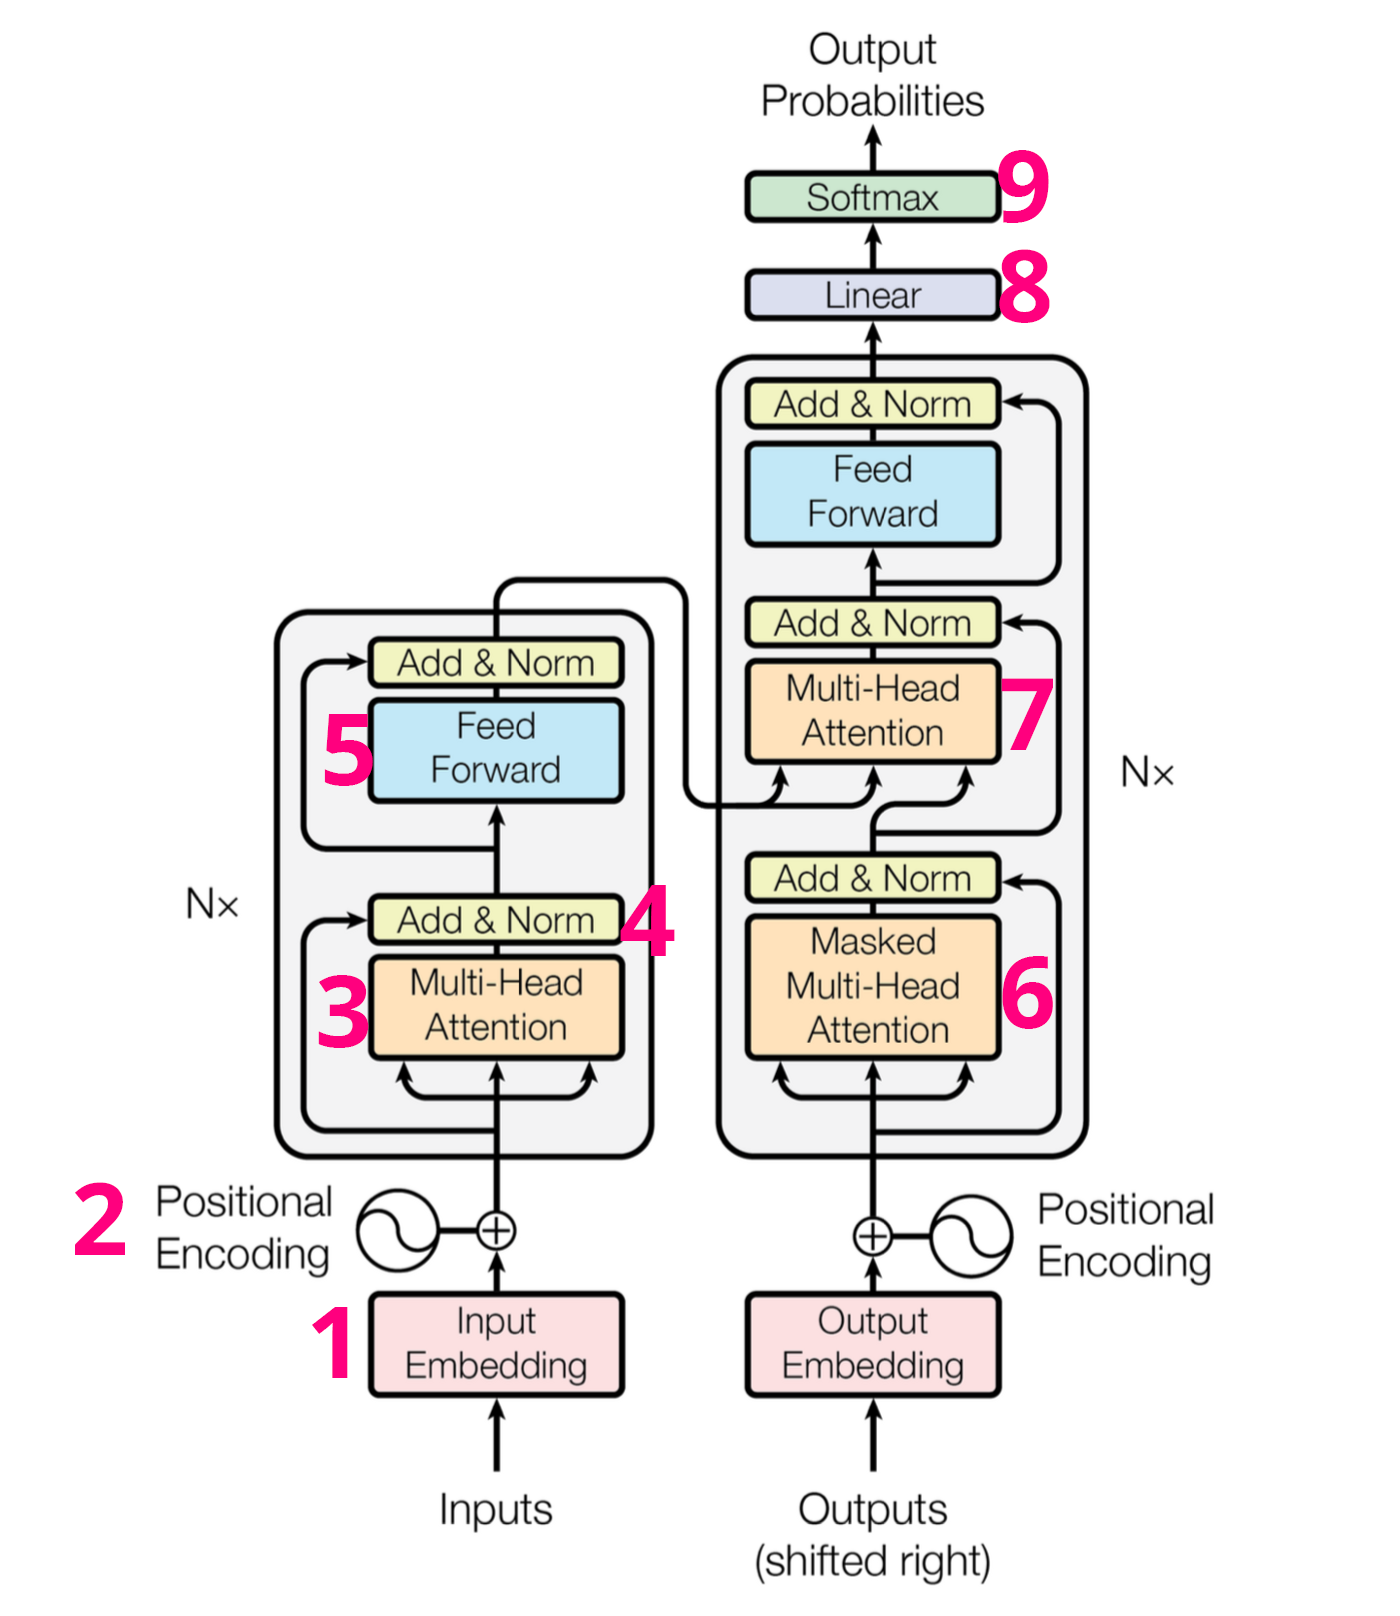
\includegraphics[width=15cm]{./img/chp2/transformerLables.png}}
\caption{The network model}\label{fig:model2}
\end{figure}


\chapter{CHAPTER 3 DESIGN AND 	METHODOLOGY}

\section{Feature Lists}

\subsection{Editor}
	Our program’s basic function is to allow users to type in texts or paste them from other sources, so the program can use these texts with other functions.

\subsection{Repetition highlights}
	As the name said. The program should highlight the repetitions for the entire text input that user gives, and to not let the user get dazzled when seeing those repetitions in case there are many repeated words in the document. Only the first word or every repetition word will be highlighted, and only shows all the repetition locations when the user hovers or clicks on it.
\subsection{Repetition replacement suggestion}

	When a user clicks on any repetition words found, a list of similar or the word that can be replaced will be shown on the UI for the user to make a decision.
\subsection{Word exception list}
	In case that user doesn’t want this specific word to be detected as a repetition whether in this document or others. They can select the word as an exception. And this list of exceptions can be decided to use in other documents, use for individual words, or not used at all.
\subsection{Use case Diagram and Sequence Diagram}

\subsection{Components and Modules}
\subsection{User Interface}
\subsubsection{Input area}
Allow user to input the text either by typing out or copy-and-paste the text.
The words that are marked as overused will be highlighted.
\subsubsection{Information area}
The side panel will be used to show additional details such as alternative words as well as their definition. 

\subsection{Text normalizer}
	The writer can either type out the text or copy and paste from somewhere else. The latter can cause problems during tokenization. One example is the apostrophe, the tokenizer expects straight quotes, if the curly variant is used, it will lead to a wrong result. The text normalizer performs token transformation to turn all the input into a compatible form supported by the tokenizer.


\subsection{Tokenizer}
Tokenizer is a task to break input text into individual components known as tokens. This is a critical step and is done before any further analysis can take place. The token can be in a form of a word or sub-word depending on the desired goal. In this project, we need several tokenizers to achieve the goal.
\subsubsection{Regex Tokenizer}
Using regular expression to match the specified pattern of the input text and then separate them into a token. Currently, the regular expression supports the following cases: 
Word matching: apple, banana, pencil
word with hyphen: plant-based, state-of-the-art, cloud
USD currency: $120, 1$
abbreviation: U.S.D., N.D.
initials containing up to 3 characters: Mr. Mrs. Ph.D.

	Unlike most out-of-the-box tokenizers which are designed to behave in a specific way, although it is easier to use, altering its behavior is nearly impossible. Some tokenizers break apart the contraction (don’t → do n’t) which is not a desirable result for our project. Instead, all contractions must remain as a single token. This is where the regex tokenizer comes in, it is very flexible and can be extended to cover most patterns the way we intended. However, one downside is the performance, some matcher uses greedy search behavior which can increase the execution speed, especially for a long text.  After weighing the pros and cons, we decided to go with a regex-based tokenizer due to its flexibility.

\subsubsection{Spacy tokenizer}
The default tokenizer shipped with the package outputs a specific format of tokens that are different from our tokenizer, for example, don’t → do and n’t. In Spacy, there are many models out of the box which we can use to perform various NLP tasks namely NER and POS, but all of them expect the token to be in this particular format. Therefore, with our regexp-based tokenizer, the output tokens are not in the right format, thus, performance suffered significantly. This is why we need to use the default Spacy tokenizer instead.

\subsubsection{BERT tokenizer}
This is a special kind of tokenizer used for BERT family tokenizer. Instead of breaking down the text into words level, this breaks down the individual word to a sub-word level. For example, Internationalization → inter \#national \#\#iz\#\#ation. The reason is to overcome the out-of-vocabulary problem. This approach is called workpiece tokenization. Each token will be converted to embedding specific to the transformer architecture. 
Note that this approach is used only in the suggestor module, not anywhere else.

\subsection{Cleaner}
This module will be used after the text has been tokenized by the tokenizer module. At this point, the tokenized text still contains stop words, for example, I, You, So, It’s, To, As, etc. These words are very common and will appear very frequently in any text regardless of the writer’s ability. Thus, counting those into the repetition list will not provide much benefit for the writer in terms of helping them avoid repetitions.

\subsection{Detector}
The role of this module is to count all the occurrences of words in the text. There are single-word or unigrams, two-word phrases or bigrams, and three-word phrases or trigrams. In NLP, this is known as ngrams. 
\subsubsection{Unigram counter}
Detect a single word occurrence in the text by counting, the common words will be filtered to keep only the meaningful words. 
\subsubsection{Bigram counter}
Detect a 2-word occurrence in the text using NLTK bigram collocation package, the quality of bigram is evaluated using association score.
\subsubsection{Trigram counter}
Detect a 3-word occurrence in the text using NLTK bigram collocation package, the quality of trigram is evaluated using association score.
\subsection{Suggestor}
The word suggestor is used to suggest an alternative word that can be substituted in the original sentence without changing the meaning of the text. 
\subsection{Candidate generation}

	Roberta is used as the main model to generate substitution candidates. The model is similar to BERT but without the next sentence prediction part, leaving with just the masking language modeling (MLM) objective. The primary task is to use MLM to fill in the masked token. For instance, I like playing video game because it is fun. Let's say we want to replace the word “fun”, we replace it with <mask> token. The sentence “I like playing video game because it is <mask> will be concatenated with the original unmasked sentence to create a sentence pair. The model attempts to predict the sentence pairs using the context clue from the original sentence with no mask. This approach is used alongside the second approach called embedding dropout which randomly set the target embedding to zero. Without the second approach, the predicted output is very likely to be the original word itself, which is not what we want. We can overcome this issue with the help of embedding dropout.

\subsection{Candidate validation}

Not all generated candidates are a suitable substitution. Although most of them fit in the context well, it changes the meaning of the original sentence entirely. The validation process contains scoring criteria based on semantic similarity between both sentences, and lexical relationships extracted from wordnet. A higher score will advance the rank, the lower score will be filtered out if it falls below the threshold.


\begin{table}[!h]
\centering
\caption{test table x1}\label{tbl:symbols}
\begin{tabular}{@{}p{0.07\textwidth}|p{0.7\textwidth}p{0.1\textwidth}}\hline
\multicolumn{2}{l}{\textbf{SYMBOL}}  & \textbf{UNIT} \\ \hline 
$\alpha$ & Test variable\hfill & m$^2$ \\
$\lambda$ & Interarrival rate\hfill &  jobs/second\\
$\mu$ & Service rate\hfill & jobs/second \\ \hline
\end{tabular}
%\begin{tabular}{c|c} \hline
% $\alpha$ & $\beta$ \\ \hline
% $\delta$ & $\mu$ \\ \hline
%\end{tabular}
\end{table}

\section{System Specifications and Requirements}

\section{Hardware Module 1}
\subsection{Component 1}
\subsection{Logical Circuit Diagram}

\section{Hardware Module 2}
\subsection{Component 1}
\subsection{Component 2}

\section{Path Finding Algorithm}

\section{Database Design}

\section{GUI Design}



%%%%%%%%%%%%%%%%%%%%%%%%%%%%%%%%%%%%%%%%%%%%%%%%%%%%%%%%%%%%%%
%%%%%%%%%%%%%%%%%%%% Experiments %%%%%%%%%%%%%%%%%%%%%%%%%%%%%
%%%%%%%%%%%%%%%%%%%%%%%%%%%%%%%%%%%%%%%%%%%%%%%%%%%%%%%%%%%%%%%
\chapter{Implementation Results}

You can title this chapter as \textbf{Preliminary Results} or \textbf{Work Progress} for the progress reports. Present implementation or experimental results here and discuss them.

%%%%%%%%%%%%%%%%%%%%%%%%%%%%%%%%%%%%%%%%%%%%%%%%%%%%%%%%%%%%%%%
%%%%%%%%%%%%%%%%%%%% Conclusions %%%%%%%%%%%%%%%%%%%%%%%%%%%%%
%%%%%%%%%%%%%%%%%%%%%%%%%%%%%%%%%%%%%%%%%%%%%%%%%%%%%%%%%%%%%%%
\chapter{Conclusions}

This chapter is optional for proposal and progress reports but 
is required for the final report.

\section{Problems and Solutions}
State your problems and how you fixed them.

\section{Future Works}
What could be done in the future to make your projects better.

%%%%%%%%%%%%%%%%%%%%%%%%%%%%%%%%%%%%%%%%%%%%%%%%%%%%%%%%%%%%%%%
%%%%%%%%%%%%%%%%%%%% Bibliography %%%%%%%%%%%%%%%%%%%%%%%%%%%%%
%%%%%%%%%%%%%%%%%%%%%%%%%%%%%%%%%%%%%%%%%%%%%%%%%%%%%%%%%%%%%%%

%%%% Comment this in your report to show only references you have
%%%% cited. Otherwise, all the references below will be shown.
%\nocite{*}
%% Use the kmutt.bst for bibtex bibliography style 
%% You must have cpe.bib and string.bib in your current directory.
%% You may go to file .bbl to manually edit the bib items.

\makeatletter
\g@addto@macro{\UrlBreaks}{\UrlOrds}
\makeatother

\bibliographystyle{kmutt}
\bibliography{string,cpe}

%%%%%%%%%%%%%%%%%%%%%%%%%%%%%%%%%%%%%%%%%%%%%%%%%%%%%%%%%%%%%%%
%%%%%%%%%%%%%%%%%%%%%%%% Appendix %%%%%%%%%%%%%%%%%%%%%%%%%%%%%
%%%%%%%%%%%%%%%%%%%%%%%%%%%%%%%%%%%%%%%%%%%%%%%%%%%%%%%%%%%%%%%
\appendix{First appendix title}
\noindent{\large\bf Put appropriate topic here} \\

This is where you put hardware circuit diagrams, detailed experimental data in tables or source codes, etc.. \\ \bigskip



This appendix describes two static allocation methods for fGn (or fBm)
traffic. Here, $\lambda$ and $C$ are respectively the traffic arrival
rate and the service rate per dimensionless time step. Their unit are
converted to a physical time unit by multiplying the step size
$\Delta$. For a fBm self-similar traffic source,
Norros~\cite{norros95} provides its EB as
\begin{equation}\label{eq:norros}
  C = \lambda + (\kappa(H)\sqrt{-2\ln\epsilon})^{1/H}a^{1/(2H)}x^{-(1-H)/H}\lambda^{1/(2H)}
\end{equation}
where $\kappa(H) = H^H(1-H)^{(1-H)}$. Simplicity in the calculation is
the attractive feature of (\ref{eq:norros}).

The MVA technique developed in~\cite{kim01} so far provides the most
accurate estimation of the loss probability compared to previous
bandwidth allocation techniques according to simulation results.
Consider a discrete-time queueing system with constant service rate
$C$ and input process $\lambda_n$ with $\mathbb{E}\{\lambda_n\} =
\lambda$ and $\mathrm{Var}\{\lambda_n\} = \sigma^2$.  Define $X_n \equiv
\sum_{k=1}^n \lambda_k - Cn$.  The loss probability due to the MVA
approach is given by
\begin{equation}\label{eq:loss_mva}
  \varepsilon \approx \alpha e^{-m_x/2}
\end{equation}
where
\begin{equation}\label{eq:mx}
m_x = \min_{n \geq 0} \frac{((C-\lambda)n + B)^2}{\mathrm{Var}\{X_n\}} =
\frac{((C-\lambda)n^\ast + B)^2}{\mathrm{Var}\{X_{n^{\ast}}\}}
\end{equation} 
and 
\begin{equation}\label{eq:alpha}
  \alpha =
  \frac{1}{\lambda\sqrt{2\pi\sigma^2}}\exp\left(\frac{(C-\lambda)^2}{2\sigma^2}\right)
  \int_C^\infty (r-C)\exp\left(\frac{(r-\lambda)^2}{2\sigma^2}\right)\, dr
\end{equation}
For a given $\varepsilon$, we numerically solve for $C$ that satisfies
(\ref{eq:loss_mva}). Any search algorithm can be used to do the task.
Here, the bisection method is used.  

Next, we show how $\mathrm{Var}\{X_n\}$ can be determined.  Let
$C_{\lambda}(l)$ be the autocovariance function of $\lambda_n$.  The
MVA technique basically approximates the input process $\lambda_n$
with a Gaussian process, which allows $\mathrm{Var}\{X_n\}$ to be
represented by the autocovariance function.  In particular, the
variance of $X_n$ can be expressed in terms of $C_{\lambda}(l)$ as
\begin{equation}
  \mathrm{Var}\{X_n\} = nC_{\lambda}(0) + 2\sum_{l=1}^{n-1} (n-l)C_{\lambda}(l)
\end{equation} 
Therefore, $C_{\lambda}(l)$ must be known in the MVA technique, either
by assuming specific traffic models or by off-line analysis in case of
traces.  In most practical situations, $C_{\lambda}(l)$ will not be
known in advance, and an on-line measurement algorithm developed
in~\cite{eun01} is required to jointly determine both $n^\ast$ and
$m_x$. For fGn traffic, $\mathrm{Var}\{X_n\}$ is equal to $\sigma^2
n^{2H}$, where $\sigma^2 = \mathrm{Var}\{\lambda_n\}$, and we can find
the $n^\ast$ that minimizes (\ref{eq:mx}) directly. Although $\lambda$
can be easily measured, it is not the case for $\sigma^2$ and $H$.
Consequently, the MVA technique suffers from the need of prior
knowledge traffic parameters.


%%%%%%%%%%%%%%%%%%%%%%%%%%%%%%%%%%%%%%%%%%%%%%%%%%%%%%%%%%
%%%%%%%%%%%%%%% The 2nd appendix %%%%%%%%%%%%%%%%%%%%%%%%%%
%%%%%%%%%%%%%%%%%%%%%%%%%%%%%%%%%%%%%%%%%%%%%%%%%%%%%%%%%%
\appendix{Second appendix title}
\noindent{\large\bf Put appropriate topic here} \\

Next, we show how $\mathrm{Var}\{X_n\}$ can be determined.  Let
$C_{\lambda}(l)$ be the autocovariance function of $\lambda_n$.  The
MVA technique basically approximates the input process $\lambda_n$
with a Gaussian process, which allows $\mathrm{Var}\{X_n\}$ to be
represented by the autocovariance function.  In particular, the
variance of $X_n$ can be expressed in terms of $C_{\lambda}(l)$ as
\begin{equation}
  \mathrm{Var}\{X_n\} = nC_{\lambda}(0) + 2\sum_{l=1}^{n-1} (n-l)C_{\lambda}(l)
\end{equation} 

\noindent{\large\bf Add more topic as you need} \\

Therefore, $C_{\lambda}(l)$ must be known in the MVA technique, either
by assuming specific traffic models or by off-line analysis in case of
traces.  In most practical situations, $C_{\lambda}(l)$ will not be
known in advance, and an on-line measurement algorithm developed
in~\cite{eun01} is required to jointly determine both $n^\ast$ and
$m_x$. For fGn traffic, $\mathrm{Var}\{X_n\}$ is equal to $\sigma^2
n^{2H}$, where $\sigma^2 = \mathrm{Var}\{\lambda_n\}$, and we can find
the $n^\ast$ that minimizes (\ref{eq:mx}) directly. Although $\lambda$
can be easily measured, it is not the case for $\sigma^2$ and $H$.
Consequently, the MVA technique suffers from the need of prior
knowledge traffic parameters. 





\end{document}
